\section{Introduction}

Generative probabilistic models are specifies probabilistic models through two mechanisms.
First, one constructs probability distributions by specifying algorithms that simulates the data generating process.
Second, one specifies assertions that condition distributions in the model.
Although the kinds of model that can be specified constructively has increased dramatically over time, whereas the kinds of statement that one can condition a model on has not.

The kinds of statement that one can condition a model on is in practice limited to a restricted form of observation of data.
In Bayesian networks, one observes a node to be a value.
While the specifics vary by formalism, the general limitation is that (i) random variables that can be conditioned must be primitive, and not derived, and (ii)

% The value of probabilistic programming systems hinges on how easily a practitioner can encode domain knowledge into a model. Existing probabilistic programming systems support two main mechanisms for encoding knowledge: implicitly in the generative model, and explicitly by conditioning on observations. There are many contexts, however, for which neither of these two mechanisms are sufficient to encode the knowledge that practitioners have about a process.
These limitations impose stringent limitations of the kinds of models that we can express.
For example, consider the problem of modeling the evolution of glucose levels over time~\citep{levine2017offline}. Using existing approaches, a scientist could define a generative model that captures prior knowledge of how glucose levels evolve over time---for example, the model may use latent variables to identify when a person eats and the glycemic loads of the meals a person consumes, and encode some physiological knowledge of how those meals will affect glucose levels. A scientist could also condition the model on concrete observations of glucose measurements on a given patient to infer the values of the latent variables in the model for that patient. However, explicitly conditioning on properties of the distribution such as ``human glucose curves are similar across patients'' is surprisingly challenging even in the most expressive probabilistic programming systems. 

In some cases it is possible to manually encode declarative knowledge constructively into a generative model.
For example, one may specify a truncated normal distribution by conditioning a normal distribution to be bounded, or constructively using the inverse transform method.
However, in most cases there is no straightforward means.
Continuing the glucose example, we may attempt to tie parameters by drawing the parameters for each patient from a shared stochastic process.
However, this increases the complexity of the generative model and requires significant expertise to ensure that the new generative model indeed captures the high-level constraint without unnecessarily constraining the model in unwanted ways.
% Moreover if the model is composed of flexible, potentially nonparametric parts, encoding anything but the simplest of constraints into the generative process becomes virtually impossible.

The primary contribution of this paper is an inference proecdure for sampling of distributioned conditioned on a larger class of statements.
To support this, in Omega we develop a new set of inference methods that work by softening predicates
over the entire probability space while preserving the distribution for those variables that meet the
constraint.

The rest of the paper proceeds as follows:
\begin{itemize}
\item We first formalize the concept of a probabilistic model as a collection of random variables defined on a shared probability space, and show how conditioning creates new probability models by chaining the probability space.  Next we define Omega: a system for building models by composing and conditioning random variables.
\item Following this, we describe our approach to inference, which softens the hard constraints as defined in measure theoretic probability to admit tractable inference in a broader set of scenarios.
\item  We demonstrate our approach on a number of examples, with experiments on toy data and experiments on medical models by enriching them with declarative knowledge to learn from limited data.
\end{itemize}

\section{Related Work}
Probabilistic programming systems~\citep{milch20071, wood2014new,mansinghka2014venture,goodman2008church,carpenter2017stan} provide a formalism
for declaring probabilistic models and performing inference
in them. Traditional probabilistic programming approaches support model definition by simulation thereby, hiding the underlying probability space. 
One exception to this is Blog \citep{milch20071} 
that defines models in terms of the generating functions.

In contrast, Omega exposes the underlying probability space and performs inference in this space as well. The value of the approach Omega takes lies in that complex random variables, functions of the probability space, can be reused to build different models by changing the underlying probability space. The exposure of the probability space incurs a cost: it is hard to compute likelihoods of random variables because they can be arbitrary transformations of fixed randomness. This means for inference in Omega we have to use likelihood-free techniques. These methods can be less efficient than their likelihood-based counterparts. Given the completeness of many probabilistic programming systems, the formalism of Omega can be implemented inside them.

Omega relates to smooth interpretation of programs \citep{chaudhuri2010smooth}.
As traditional computer programs are collections of predicates, the techniques used to soften predicates for inference in Omega can also be used to build systematic smooth approximations of these programs. Similarly, tools from smooth interpretation can be used to build new kinds of inference algorithms.

% \begin{itemize}
% 	\item Probability is important
%     \item Using probability can be hard (e.g., posterior computation)
%     \item Important for widespread probabiltiy, mental model needs to match formal semantics
%     \item Systems like Stan have made things easier, but the notion of conditioning and expressing weak knowledge requires the user to bake into  a generative process
%     \item Contrast constructive generative model with declarative knowldege you condition on
%     \item "Conditioning is declaring knowledge sentence you have" 
%     \item Motivating examples \textbf{Need to think about simplest example}
%  	\item We formalize the notion of declarative knowledge
%     \item We provide a syntex and sematics
%     \item We develop inference algorithms for both when the knowledge is hard and when it's soft (either for compute or because there's uncertainty about the knowledge)
%     \item Just like inference can be abstracted, model building can be as well
% \end{itemize}

% !TEX root = nips_2018.tex

\section{Simulation Models}\label{simmodels}


% The density function of the resulting model, if it exists, is not explicitly represented, but rather implicitly defined.
% For this reason simulator models are often called implicit or generative models.

% Simulator-based models are useful because they interface easily with models typicallyencountered in the natural sciences. In particular, hypotheses of how the observed datayowere generated can be implemented without making excessive compromises in order tohave an analytically tractable model

Probabilistic simulation based models specify the step-by-step causal mechanisms of a domain, and use probability distributions for any uncertain parameters.
A simulation model can be stochastically executed, using a random number generator to sample from primitive random variables in the model.
Inference means to simulate the model while imposing constraints on variables in the model.
This is difficult, since simulation based models lack an explicit likelihood function, which is necessary for most inference procedures.

Conditioning on predicates requires a measure-theoretic foundation, in which a simulation model is a random variable:

\begin{figure}
	\centering
	\begin{minipage}[t]{5cm}
		\centering
		
\includegraphics[width=0.45\linewidth]{figures/clunk}
		% \begin{verbatim}
		%         rand(objs)
		% \end{verbatim}
	\end{minipage}%
	\begin{minipage}[t]{5cm}
		\centering
		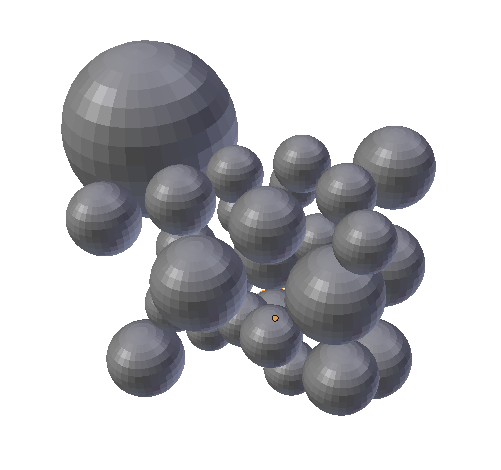
\includegraphics[width=0.45\linewidth]{figures/render}
		% \begin{verbatim}
		% pred = nointersect(objs)
		% rand(scene, pred)
		% \end{verbatim}
	\end{minipage}%
	% \begin{minipage}[t]{5cm}
	% \centering
	% 
\includegraphics[width=0.5\linewidth]{figures/equi}
	% $$
	% x = 3
	% $$
	% % \begin{verbatim}
	% % pred = equidistant(objs)
	% % rand(scene, pred)
	% % \end{verbatim}
	% \end{minipage}
	\caption{A weak prior (left) does not respect rigid body constraints on objects, whereas (center) is conditioned on the predicate that objects don't intersect.  (right) objects are conditioned on being equidistant, resulting in a tetrahdral arrangement}
	\label{fig:nointersect}
\end{figure}


\paragraph{Random Variables.} Probability models lie on top of probability
spaces. A probability space is a measure space $(\Omega, {\cal H}, {\cal P})$,
where ${\cal H}$ is a sigma algebra and ${\cal P}(\Omega) = 1$ \citep{ccinlar2011probability}. Random variables are
functions from the space $\Omega$ to a realization space ${\cal X}$. As a concrete
example the space $\Omega$ can be thought of as a hypercube, with ${\cal P}$ being
uniform over that hypercube. To build a normal random variable, we need a function
that maps from $\Omega \to \mathbb{R}$. If the underlying probability space is uniform, then
this function is the inverse cumulative distribution function of the normal.

A \emph{model} $\cM$ is a collection of random variables along with a probability space.
% To fully specify a model, we need both the measure space and the
% collection of random variables on which it acts.

\paragraph{Conditioning}

Conditioning a model creates a new model.
As an example consider a model $\cM$ with two
random variables $X_1$ and $X_2$ that both take real values. Conditioning
$\cM$ on $X_1 = 1$, defines a new model $\cM_{|A}$ based on limiting the measure space
$\Omega$ to the set $A = \{ \omega : X_1(\omega) = 1\}$.
The new model is defined on a new probability space
\begin{align}
	(\Omega \cap A, \{A \cap B, B \in {\cal H} \}, {\cal P} / {\cal P}(A))
\end{align}
with the same random variables $X_1$ and $X_2$.
Sampling from $\cM_{|A}$ produces
samples only where $X_1 = 1$

More generally, conditioning on any predicate $Y(\omega) = \lk(X_1(\omega), \dots, X_n(\omega))$
defines a new model defined exactly as above, where $A = \{\omega : \lk(X_1(\omega), \dots, X_n(\omega)) = 1\}$.
% This predicate may include a comparisonsuch as $X_i < X_j$, restrict deterministic function of variables in in the model such as $\exp(X_i) = 2$, or be a Boolean combination such as $(X_i < X_j) \lor \neg(\exp(X_i) = 2)$.
Sampling from $\cM_{|A}$ generates $(x_1, ..., x_n)$ where $\lk$ is true.

The general construction of new models might require conditioning
on sets of measure zero. This process can be made rigorous
via disintegration \citep{chang1997conditioning}. Disintegration can
be thought of as the reversal of building joint distributions through
product measure constructions.


% When building models with prior beliefs via conditioning, we would like
% the property that given an infinite collection of observations, the 
% posterior predictive distribution converges to true sampling distribution.
% To study this, consider a model with two random variables that are independent,
% $X_1$ is a function of $\omega_1$ and $X_2$ is a function of $\omega_2$. Suppose
% that the true sampling distribution has $X_1$ and $X_2$ positively correlated.
% For the prior beliefs to support positive correlations, we 
% could condition on a prior belief that $X_1$ and $X_2$ are close. However
% if the form of the closeness isn't controlled by a random variable, observing
% an arbitrary amount of data from the true distribution will not change
% the dependence between $X_1$ and $X_2$ in the model. 
% \begin{align*}
% X_j^*(\omega^*) = \sigma(f_\Beta(X_{j, 1}, ..., X_{j, n})) > b, \\
% \end{align*}
% Conditioning on $X_j^*$ produces a new set of models that have 
% dependence between . Knowledge is encoded in the prior distribution
% on $\Beta$. If $f_\Beta$ has priors over the true dependence between
% $X_{., 1},...,X_{., m}$, then this new model family will converge
% to the true underlying distribution.

% rr: TODO the above can me made into a proof

% \subsection{Bayesianism vs. Bayesian Computation}
% The way we 


% \section{Higher Order Random Variables}
% People often entertain beliefs about probability statements. For instance most people accept 
% trust expert-given odds that a particular sports team will win a tournament, 
% or politician will win an election, more than the odds of those given by non-experts.
% The apparent failure of probabilistic expressions to distinguish 
% between these cases led to alternative formalisms of uncertainty \citet{Shampher}, 
% but within the probabilistic framework both \citet{Pearl} and \citet{Hyberg} demonstrated 
% that such higher order distributions were induced from the original model, no new machinery was needed.

% As a concrete example of this, suppose we have a stochastic 
% dynamical system model of human blood glucose 
% controlled by some 
% parameters $\Theta$ with a prior. A priori we know that the average blood pressure 
% in a person lives in a physically plausible range $40-400$. A way to
% encode this would be to change the prior on the parameters $p(\Theta)$ 
% to so that any sample from that prior yields has average in the physically
% plausible range. This can be challenging because it requires a detailed
% understanding of the stochastic dynamical system. 

% Alternatively, we could try to take the conditioning approach from the
% previous section. But conditioning in the previous section required explicitly
% defined random variables, and while the average glucose is a random variable
% because the parameter $\Theta$ is random, it is not an explicit random variable.
% The scenario requires the ability to both define and condition on 
% probability distributions over either random variables or properties of 
% random variables (e.g. expectations).
% In this section we introduce the random conditional 
% distribution ($\randcond$) to support this task.

% \paragraph{The Random Conditional Distribution.}
% The random conditional distribution of $X$ given $\Theta$ -- which we denote $\rcd(X, \Theta)$ or $\rcdxy{X}{\Theta}$ -- is a random distribution: a random variable which takes values in the domain of random variables.
% Informally, $\rcdxy{X}{\Theta}$ is a function of $\omega$ that returns functions of $\omega$
% of the same type as $X$. Formally, $\rcd$ is a distribution over conditional random variables:

% % The primary mechanism for conditioning is $\cond$, which constructs conditional random variables:
% % \begin{definition}
% % Let $X:\Omega \to T$ be a random variable, $Y$ an indicator function, and $\conds{X}{Y}: \Omega_{|Y} \to T$ be a conditional random variable defined as: $X_{|Y}(\omega) = X(\omega)$.
% % $X_{|Y}$ is defined on a conditioned probability space $(\Omega, \Sigma, \mu_{|Y})$ where $\mu_{|Y}$ is a conditional measure: $
% % \mu_{|Y}(A) = \mu(A \cup Y^{-1}(\{1\})) / \mu(Y^{-1}(\{1\})$.
% % % That is, $\cond: (\Omega \to T) \times (\Omega \to \{0, 1\}) \to (\Omega \to T)$ is a operator that restricts the domain of $X$ to those inputs consistent with $Y$.
% % \end{definition}


% \begin{definition}The random conditional distribution of a random variable $X: \Omega \to T_1$ given $\Theta: \Omega \to T_2$ is a random variable $\rcdxy{X}{\Theta}: \Omega \to (\Omega \to T_1)$, defined as:
% \begin{equation}\label{eq:rcd}
% (\rcdxy{X}{\Theta})(\omega) = [\conds{X}{\Theta = \Theta(\omega)}]
% \end{equation}
% \end{definition}
% For example if $\Theta = \bern(0.4)$ and $X = \normal(\Theta, 1)$, then $\rcdxy{X}{\Theta}$ is a random distribution 
% whose domain comprises of two normal distributions $X_1 = \conds{\normal(\Theta, 1)}{\Theta = 1}$ and $X_2$.
% The probabilities of $X_1$ and $X_2$ with respect $\rcdxy{X}{\Theta}$ are determined by the prior probabilities of the different outcomes of $\Theta$: $P((\rcdxy{X}{\Theta}) = X_1) = 0.4$ and $P((\rcdxy{X}{\Theta}) = X_2) = 0.6$.

% A random conditional distribution is most useful in combination with other functions.
% Expectation is perhaps the most important example, which when composed with $\rcd$ produces conditional expectation.
% Restricting to real valued variables, expectation $E$ is a functional that maps a random variable to a real value
% (($\Omega \to \mathbb{R}) \to \mathbb{R}$).
% When $X$ is a real valued random variable, $\rcdxy{X}{\Theta}$ is not real valued, and hence not a valid argument to $E$.

% However, just as arithmetic operations such as $+$ and $-$ extend from the domain of numbers to the domain of random variable (pointwise $X + Y = \omega \mapsto X(\omega) + Y(\omega)$), $E$ extends from the domain of random variables to the domain of random variables over random variables in precisely the same way.
% % Since random variables are themselves functions, $E$ is an operator, functional or more generally a higher-order function.  
% % As described in section X a function with domain $T$ can be lifted to a functional of $T$-valued random variables.
% % $T$ is purposefully left abstract, because in addition to lifting functions defined on the reals etc, we can lift functions defined on random variables.
% % Expectation is a cannonical example of a random variable valued function, with type $E : (\Omega \to \mathbb{R}) \to \mathbb{R}$.
% That is, $\ee$ has a lifted counterpart $\lifted{\ee} = \lift(\ee)$ with type $\lifted{\ee} : (\Omega \to (\Omega \to \mathbb{R})) \to (\Omega \to \mathbb{R})$, which maps a distribution over real valued random variables to a distribution over real values (expectations).
% % $$
% % \lifted{\ee}(X)(\omega) = \mean{X(\omega)}
% % $$
% The operator $\rcd$ composed with $\ee$ constructs conditional expectation (with respect to a random variable $\Theta$):
% \begin{equation}
% \lmean{\rcdxy{X}{\Theta}} = \lmean{\omega \mapsto \conds{X}{\Theta = \Theta(\omega)}} 
%                     = \omega \mapsto \mean{\conds{X}{\Theta = \Theta(\omega)}}\\
% \end{equation}
% The final term $\omega \mapsto \mean{\conds{X}{\Theta = \Theta(\omega)}}$ matches the definition of
% conditional expectation
% with respect to a random variable $\mean{(X\mid \sigma (Y))(\omega)} = \mean{X \mid Y = Y(\omega))}$.
% That is the conditional expectation is a random variable with randomness provided by the conditioning set.

% Returning to the blood glucose example, we can build a model that respects the valid range
% of average blood glucose by taking the original model creating the conditional expected
% value of glucose $G$ with $\rcd$ and expectation of $\rcd$, then constructing a new model
% by conditioning the original on $G$ being in the physiologically possible range.

% \paragraph{Completeness.}Nested uses of $\rcd$ lead to a completeness result. State informally: 
% by repeatedly applying $\rcd$, any random function or functional in the original model
% can be constructed. Then by using conditioning to create new models from the previous 
% section, we can alter existing models to respect predicates on any random quantity in
% the model even if the random quantity is not an explicit random variable.
% % RR: TODO: The above could be a theorem


%% \section{Higher Order Probabilistic Inference}

% People often entertain beliefs about probability statements.
% For instance most people accept even expert-given odds that a particular sports team will win a tournament, or politician will win an election, with a degree of scepticism.
% % and therefore (iii) perhaps we need a new or extended theory of probability to be able to reason about these facts.
% The apparent failure of probabilistic expressions to distinguish between these cases led to alternative formalisms of uncertainty \cite{Shampher}, but within the probabilistic framework both Pearl \cite{} and HyBerg{} demonstrated that such higher order distributions were induced from the original model, no new machinery was needed.
% Many scenarios require the ability to both define and condition probability distributions over either random variables or properties of random variables (e.g. expectations).
% In this section we introduce the random conditional distribution ($\randcond$) to support this task.
% $\rcd$ is best explained through example:


% % Higher order probabilities emerge whenever there is a distinction between subjective and objective probabilities.
% % For example many systems which verify probabilistic statements make assertions such as this assertion holds with a probability greater than 0.9.
% % This distinction between the objective probability with which the assertion holds and the bound that can be proved reflects the gap in the reasoning capacity of the agent.

% % Further still, higher order distributions is a more general concept that higher order probabilities, encompassing it as a special case.
% % Consider an assertion about the fairness of a hiring program $P$ that takes as input a vector of arguments $v$ representing a job applicant’s record and returns a Boolean value indicating whether the applicant is hired.
% % One of the arguments $v$ 


% Consider a coin toss in the basement of a unscrupulous gambler, and having the belief that the coin could be fair or be biased towards tails, but also that the coin-tosser may bias its outcome through sleight of hand.

% \begin{figure}[!htb]
% \centering
% 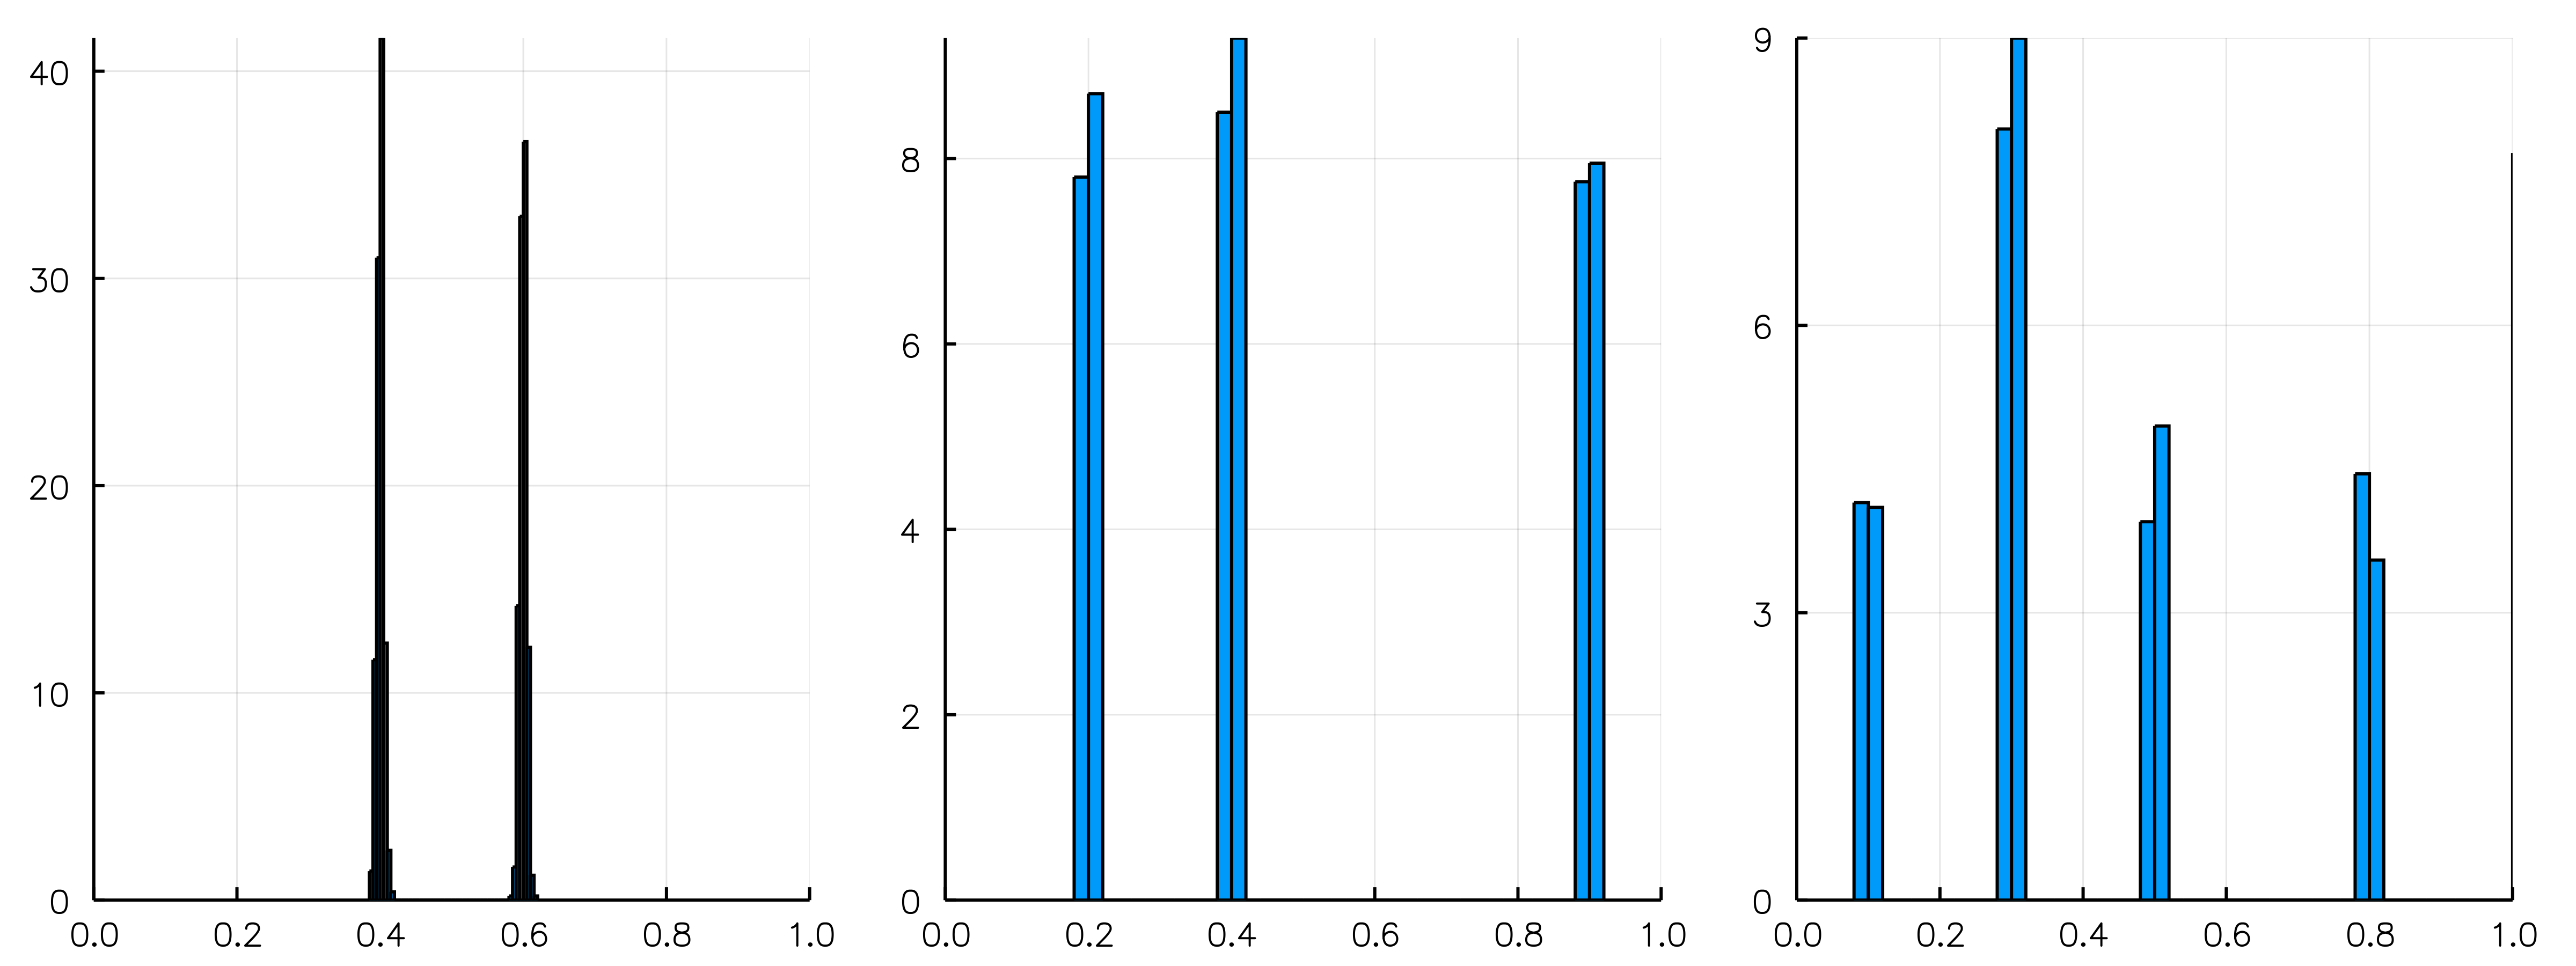
\includegraphics[width=0.9\linewidth]{figures/rcd}
% \caption{Imagine observing the outcome of flips of a coin of unknown fairness, e.g., $coin = \bern(w + b)$ comes up heads with probability $W + b$, where weight $w = \unif(\{-0.2, 0, 0.2\})$ is uniformly distributed,  $b = \unif(\{-0.2, 0, 0.5\})$
% The marginal probability that the $P(coin = H) = 0.5$ is equal to that of a bank-minted, fairly-tossed coin.
% Put another way, despite the fact that a gamblers coin tossed by untrustworthy tosser and a freshly minted coin have the same overall probability of turning up heads, we would not be very surprised if the fraction of heads appearing in a large number of the gambler coin tosses deviated greatly from 0.5, but very surprised if it occurred with bank coin tosses.
% The random conditional distribution allows us -- among other things -- to induce distributions over probabilities directly from the original model, distinguishing these two scenarios.
% \ref{rcd} demonstrates .  From left to right random samples from (a) $\mean{\rcd(coin, fair)}$, (b) $\mean{\rcd(coin, b)}$ (c) $\mean{\rcd(coin)}$}
% \label{fig:rcd}
% \end{figure}

% TODO: Higher order more general that reasoning over beliefs





% \subsection*{Lifting}
% Lifting is a process which gives meaning to expressions such as $X+X$ when $X$ is a random variable rather than a number.
% To lift a function (such as $+$) means to It constructs a functional defined on $T$-valued random variables from a function defined on values of type $T$, mechanising the principle that a transformation of a random variable yields a random variable.
% Lifting is important because syntactically, it is more convenient to use random variables as if they were values rather than compose functions in measure theoretic notation.
% In addition, it allows us to repurpose existing programs expressed in values of type $T$ (e.g., ray-tracers which take geometric objects as input) to $T$-valued random variables (distributions over objects), without modification.

% To treat random variables as values we interpret operations on them \emph{pointwise}.
% % Given a function $f$ with domain $T$, we lift it to the domain of a random variable of codomain $T$.
% Let $X:\Omega \to T_1$ be a random variable, and $f:T_1 \to T_2$ be a function, then $Y = f(X)$ is a random variable defined as:
% $$
% Y(\omega) = f(X(\omega))
% $$
% Lifting extends to multivariate functions in the obvious way, e.g.:
% $$
% X + X = \omega \mapsto X(\omega) + X(\omega)
% $$
% More generally lifting is performed through an operator $\lift$:
% \begin{definition}
% Let $f: T_i \times \cdots \times T_n$ be an $n$-ary multivariate function, and denote by $e_\omega()$ the evaluation functional defined by $e(X, \omega) = x(\omega)$ if $X$ is a random variable and $e(X, \omega) = X$ otherwise.
% $\lifted{f}: (\omega \to T_1) \times \cdots \times (\omega \to T_n)$ where $f(X)$
% \end{definition}

% \improvement{WHY is lifting defined pointwise}

% \subsection*{Conditional Random Variable}
% Probabilistic inference is achieved through conditioning.
% To condition means to restrict the universe to only those scenarios where a condition holds.
% A predicate $Y: \Omega \to \{0,1\}$ can be used to restrict a probabilistic model to a subset of the uncertainty.
% That is, every event $A$ has a characteristic predicate $Y$ defined by
% $Y(\omega) = 1$ if $\omega \in A$, otherwise $Y(\omega) = 0$.
% Equivalently, the image of $A$ under $Y$ is $\{1\}$ and the preimage of $\{1\}$ under $Y$ is $A$ is 
% $Y^{-1}(\{1\}) = \{ \omega \in \Omega : Y(\omega)\} = A$

% The primary mechanism for conditioning is $\cond$, which constructs conditional random variables:
% \begin{definition}
% Let $X:\Omega \to T$ be a random variable, $Y$ an indicator function, and $X_{|Y}: \Omega_{|Y} \to T$ defined as $\cond(X, Y)$ be a conditional random variable defined as: $X_{|Y}(\omega) = X(\omega)$.
% $X_{|Y}$ is defined on a conditioned probability space $(\Omega, \Sigma, \mu_{|Y})$ where $\mu_{|Y}$ is a conditional measure: $
% \mu_{|Y}(A) = \mu(A \cup Y^{-1}(\{1\})) / \mu(Y^{-1}(\{1\})$.
% That is, $\cond: (\Omega \to T) \times (\Omega \to \{0, 1\}) \to (\Omega \to T)$ is a operator that restricts the domain of $X$ to those inputs consistent with $Y$.
% \end{definition}

% Conditional random variables.  Operations on conditional random variables constructs further conditional random variables.
% Observe that if two conditional random variables are composed then:

% $$
% \begin{aligned}
% (f(X_{|Y}))(\omega)&=f(X_{|Y}(\omega))&{\text{ where } Y(\omega)}\\
% (f(X_{|Y_1}, X_{|Y_2}))(\omega)&=f(X_{|Y}(\omega))&{\text{ where } Y_1(\omega)} \wedge Y_2(\omega)\\
% % (\lambda f)(x)&=\lambda \cdot f(x)&{\text{(pointwise multiplication by a scalar)}}
% \end{aligned}
% $$

\section{The Random Conditional Distribution}
The random conditional distribution of $X$ given $\Theta$ -- which we denote $\rcd(X, \Theta)$ or $\rcdxy{X}{\Theta}$ -- is a random distribution: a random variable which takes values in the domain of random variables.
Informally, $\rcdxy{X}{\Theta}$ is a probability distribution over random variables of the same type as $X$, where each random variable in that distribution corresponds to an element of $\theta \in \Theta$ and is weighted by the prior probability of $\theta$.
Formally, $\rcd$ is a distribution over conditional random variables:

% The primary mechanism for conditioning is $\cond$, which constructs conditional random variables:
\begin{definition}
Let $X:\Omega \to T$ be a random variable, $Y$ an indicator function, and $\conds{X}{Y}: \Omega_{|Y} \to T$ be a conditional random variable defined as: $X_{|Y}(\omega) = X(\omega)$.
$X_{|Y}$ is defined on a conditioned probability space $(\Omega, \Sigma, \mu_{|Y})$ where $\mu_{|Y}$ is a conditional measure: $
\mu_{|Y}(A) = \mu(A \cup Y^{-1}(\{1\})) / \mu(Y^{-1}(\{1\})$.
% That is, $\cond: (\Omega \to T) \times (\Omega \to \{0, 1\}) \to (\Omega \to T)$ is a operator that restricts the domain of $X$ to those inputs consistent with $Y$.
\end{definition}


\begin{definition}The random conditional distribution of a random variable $X: \Omega \to T_1$ given $\Theta: \Omega \to T_2$ is a random variable $\rcdxy{X}{\Theta}: \Omega \to (\Omega \to T_1)$, defined as:
\begin{equation}\label{eq:rcd}
(\rcdxy{X}{\Theta})(\omega) = \conds{X}{\Theta = \Theta(\omega)}
\end{equation}
\end{definition}
For example if $\Theta = \bern(0.4)$ and $X = \normal(\Theta, 1)$, then $\rcdxy{X}{\Theta}$ is a random distribution comprised of two normal distributions $X_1 = \conds{\normal(\Theta, 1)}{\Theta = 1}$ and $X_2$.
The probabilities of $X_1$ and $X_2$ with respect $\rcdxy{X}{\Theta}$ are determined by the prior probabilities of the different outcomes of $\Theta$: $P((\rcdxy{X}{\Theta}) = X_1) = 0.4$ and $P((\rcdxy{X}{\Theta}) = X_2) = 0.6$.

A random conditional distribution is most useful when used in combination with other functions.
Expectation is perhaps the most important example, which when composed with $\rcd$ produces conditional expectation.
Expectation $E : (\Omega \to \mathbb{R}) \to \mathbb{R}$ is a functional that maps a random variable to a real value.
When $X$ is a real valued random variable, $\rcdxy{X}{\Theta}$ is not real valued, and hence not a valid argument to $E$.
However, just as arithmetic operations such as $+$ and $-$ extend from the domain of numbers to the domain of random variable (pointwise	 $X + Y = \omega \mapsto X(\omega) + Y(\omega)$), $E$ extends from the domain of random variables to the domain of random variables over random variables in precisely the same way.
% Since random variables are themselves functions, $E$ is an operator, functional or more generally a higher-order function.  
% As described in section X a function with domain $T$ can be lifted to a functional of $T$-valued random variables.
% $T$ is purposefully left abstract, because in addition to lifting functions defined on the reals etc, we can lift functions defined on random variables.
% Expectation is a cannonical example of a random variable valued function, with type $E : (\Omega \to \mathbb{R}) \to \mathbb{R}$.
That is, $\ee$ has a lifted counterpart $\lifted{\ee} = \lift(\ee)$ with type $\lifted{\ee} : (\Omega \to (\Omega \to \mathbb{R})) \to (\Omega \to \mathbb{R})$, which maps a distribution over real valued random variables to a distribution over real values (expectations).
$$
\lifted{\ee}(X)(\omega) = \mean{X(\omega)}
$$
$\rcd$ composed with $\ee$ constructs conditional expectation (with respect to a random variable $\Theta$):
\begin{equation}
\lmean{\rcdxy{X}{\Theta}} = \lmean{\omega \mapsto \conds{X}{\Theta = \Theta(\omega)}} 
                    = \omega \mapsto \mean{\conds{X}{\Theta = \Theta(\omega)}}\\
\end{equation}
The final term $\omega \mapsto \mean{\conds{X}{\Theta = \Theta(\omega)}}$ is the definition of a conditional expectation with respect to a random variable $\mean{(X\mid \sigma (Y))(\omega)} = \mean{X \mid Y = Y(\omega))}$.

% Move to appendix?
% Equation \ref{eq:rcd} is a construcive definition of $\rcd$; here we define it declaratively:
% Let $\mu_\Theta = \mu \circ \Theta^{-1}$ denote the push forward measure of		 $\mu$ with respect to $\Theta$, $\tilde{X} = \randcond(X, \Theta)$, and $X^* \subset \tilde{X}$ be a set of random variables, then:
% $$
% \mu_{\tilde{X}}(X^*) = \mu_\Theta(\varphi^{-1}(X^*))
% $$

\improvement{This needs to be made clearer. Will there be issues taking measures in function space?}

\improvement{Need to define space of functions that measures exist on. Then define curry(X, $\Theta$), random variable on functions, to take measure given by pullback to $\Theta$ }

\improvement{Define: RCD of one argument $\rcd(X)$}

% \subsection{Higher Order Graphical Model}

% Probabilistic inference means to construct and condition random variables.
% In measure theory, a random variable is a function from a sample space $\Omega$ to $T$, where $T$ could for example be $\mathbb{R}$, but any type in general.
% $\Omega$ is understood as the universe of possible scenarios that could occur, or in sampling terms, as the random inputs to a random variable.
% Measure theory formalizes uncertainty by assigning probabilities to sets of possible scenarios, called events.
% The measure of an event represents a degree of belief that the event could occur, and is determined by a probability measure $\mu:\Sigma \rightarrow [0,1]$ where $\Sigma$ is a sigma-algebra (measurable subsets of $\Omega$).
% An event $A$ is impossible if $\mu(A)=0$, and certain if $\mu(A)=1$.

% We formulate $\rcd$ with respect to a form of directed graphical model.
% Higher order directed graphics are similar to standard bayesian networks but depart from them in two significant ways.
% First, the semantics of a graph is defined in terms of measure theoretic random variables, in contrast to probability mass or density functions, which means that every node is a deterministic transformation and all randomness is considered external to the system.
% Second this graph formalism is based on measure theoretic probability.

% \begin{definition}
% A higher order Bayesian Network $\mathcal{G}(V,E)$ is a directed acyclic graph, where $V$ are the nodes and $E$ are the edges of the graph.
% Nodes correspond to random variables, measurable functions from a sample space $\Omega$ to some output type $T$.
% Let $V_{\omega} \subseteq V$ denote the subset of variables without parents.
% Higher order graph are able to express both functions between  variables and functions of variables.
% Standard (non higher order) models are expressed using edges in $E_\circ$ (read $E$ compose).
% A composition edge from $A$ to $B$ denotes that $B$ functionally (and causally) depends on $A$.
% More precisely $A \to B$ denotes the composition $B \circ A$.
% Since $A$ is random variable, this composition is a random variable $\omega \mapsto B(A(\omega))$.
% \end{definition}
% Application edges in $E_{apply}$ denote function application.
% If a node $A$ is at the source of a directed edge in $E_{apply}$ it is taken as a value to be given as input to the node at the tail.
% % Let $f : V \to what$ map each node to a corresponding function, and $id : V_{\omega} \to \mathbb{N}$ map each parent-free node to a unique integer.
  
% \begin{align*}
% \mu &= \mathcal{N}(0, 1) \\
% X &= \mathcal{N}(\mu, 1) \\
% \tilde{X} &= \mathbb{E}(\rcdxy{X}{Y})
% \end{align*}


% \subsection{Efficient Construction of the Random Conditional Distributions}

Each outcome of a random conditional distribution is a conditional random variable which, in the general setting, can be a challenge to sample from.
In this section we demonstrate how to efficiently construct the random conditional distribution in a wide class of scenarios.

Recall that $(\rcdxy{X}{\Theta})(\omega) = \conds{X}{\Theta = \Theta(\omega)}$.
A realization $\conds{X}{\Theta = \Theta_c}$ of $\rcdxy{X}{\Theta}$ is a conditional random variable which may be difficult to sample from.
Instead, under modest conditions (theorem \ref{thm:path}) it is permissible to use a different distribution which is easier to construct:  $\ridxy{X}{\Theta}$ which \emph{fixes} rather than conditions $\Theta$:
\begin{equation}\label{eq:rid}
(\ridxy{X}{\Theta})(\omega) = \conds{X}{\Theta^a = \Theta^a(\omega) \text{ for all } \Theta^a \in \{ \Theta \} \cup \text{ancestors of } \Theta}
\end{equation} 
$\rcdxy{X}{\Theta}$ is distinct from $\ridxy{X}{\Theta}$ because in the former the parents of $\Theta$ are not fixed and hence for some realization $\conds{X}{\Theta = \Theta_c}$ we must consider all the possible scenarios which would result in $\Theta = \Theta_c$.
In contrast, 
$\ridxy{X}{\Theta}$ is always efficient to construct:

\begin{algorithm} 
\end{algorithm}

It is permissible to use $\ridxy{X}{\Theta}$ as a substitute for $\rcdxy{X}{\Theta}$ when they are equivalent, which is not always the case, consider:
\begin{align*}
\alpha &= \rade(0.5) \\
\beta &= \bern(0.5) * \alpha \\
\gamma &= \bern(0.5) + \alpha + \beta
\end{align*}

Random conditional distributions (such as $\rcdxy{\gamma}{\beta}$) can be induced from this model which are not equal to the corresponding "fixed" random conditional distribution: $\ridxy{\gamma}{\beta}$.
For example the distribution over expectations $\lmean{\rcdxy{\gamma}{\beta}}$ and $\lmean{\ridxy{\gamma}{\beta}}$ do not even have the same support.
However in other scenarions they are the same, e.g. $\rcdxy{\gamma}{\alpha} = \ridxy{\gamma}{\alpha}$.

Verifying equivalence of two random variables (let alone two random distributions) is undecidable in theory \ref{} and intractable in practice, putting us at risk of swapping one hard problem for a harder one.
Fortunately, the causal structure of the model provides sufficient (but not neccesary)ee conditions to determine if $\ridxy{X}{\Theta} = \rcdxy{X}{\Theta}$:
% Intuitively, the first result can be substitued because it sucks, while the seon dosn't suck.

\todo{Maybe use d-separation. $\Theta$ d-separates $X$ from its ancestors}
\begin{theorem} $\rcdxy{X}{\Theta} = \ridxy{X}{\Theta}$ when all paths from the ancestors $\Theta$ to $X$ pass through $\Theta$
\end{theorem}
\begin{proof}
To prove this theorem, it is crucial to formalize the structural assumption. The ancestors of $\Theta$ have no path to $X$ that doesn't pass through $\Theta$. This means that conditioned on $\Theta$, any ancestor of $\Theta$, $\Theta^a$, is independent from $X$, i.e.
\begin{equation*}
\conds{X}{\Theta, \Theta^a} = \conds{X}{\Theta} \quad \text{for all } \Theta^a \in \text{ancestors of } \Theta
\end{equation*}
Therefore, using \eqref{eq:rid} we obtain the following identity for all $\omega$
\begin{equation*}
(\ridxy{X}{\Theta})(\omega) = (\conds{X}{\Theta = \Theta(\omega), \Theta^a = \Theta^a(\omega) \text{ for all } \Theta^a \in \text{ancestors of } \Theta}) = \conds{X}{\Theta = \Theta(\omega)}
\end{equation*}
which concludes the proof that $\rcdxy{X}{\Theta} = \ridxy{X}{\Theta}$.
\end{proof}

% For example, to construct a set of samples from $\mean{\rcdxy{X}{Y}}$, we could:
% \begin{itemize}
% \item Unconditionally sample $Y$ to yield $y_c$.
% \item Sample $X^*$ from $\tilde{X}$ such that $X^* = X \mid Y = y_c$, where $y_c = Y(\omega_c)$ is a realization of $Y$
% \item Find $\Omega^* \subset \Omega$ such that $Y(\omega^* \in \Omega^*) = y$
% \item Compute $\mean{X^*}$ with respect to $\Omega^*$
% \end{itemize}

% Step 2 is hard for all the same reasons that conditioning is hard in general.
% However, we can exploit the fact that the condition $Y = Y(\omega)$ in $\rcdxy{X}{Y}$ is not an arbitrary condition, in effect, it is conditioning on the prior.

% \begin{itemize}
%   \item Unconditionally sample $Y$ to yield $y_c$, cache its input $\omega_c$ (i.e., $Y(\omega_c) = y_c$)
%   \item Compute $\mean{X}$ 
% \end{itemize}

% This sequence is identical in distribution to the first sequence, but dramatically easier to compute.

